\section{Anwendungen in der anorganischen Chemie}
\subsection{$^{31}$P chemische Verschiebungen in Phospor NHCs}
\ac{nhc}
\begin{figure}[ht!]
	\centering
	\includegraphics[width=0.6\textwidth]{1}
	\captionsetup{figurewithin = chapter}
	\captionsetup{font=small, labelfont=bf}\caption[Abbildung von SIMesPH]{Abbildung von SIMesPH, SIMes=1,3-bis(2,4,6-tri\-me\-thyl\-phe\-nyl)imi\-da\-zo\-lin-2-yli\-den (Kohlenstoff=grau, Wasserstoff=weiß, Stickstoff=blau und Phosphor=orange).}
\label{abb:cvh1}
\end{figure}

\begin{figure}[ht!]
	\centering
	\includegraphics[width=0.6\textwidth]{2}
	\captionsetup{figurewithin = chapter}
	\captionsetup{font=small, labelfont=bf}\caption[Abbildung von IMesPH]{Abbildung von IMesPH, IMes=1,3-bis(2,4,6-tri\-me\-thyl\-phe\-nyl)imi\-da\-zol-2-yli\-den (Kohlenstoff=grau, Wasserstoff=weiß, Stickstoff=blau und Phosphor=orange).}
\label{abb:cvh2}
\end{figure}

\begin{figure}[ht!]
	\centering
	\includegraphics[width=0.6\textwidth]{3}
	\captionsetup{figurewithin = chapter}
	\captionsetup{font=small, labelfont=bf}\caption[{Abbildung von $[$SIMesPGa\textit{t}Bu$_2]_2$}]{Abbildung von $[$SIMesPGa\textit{t}Bu$_2]_2$, SIMes=1,3-bis(2,4,6-tri\-me\-thyl\-phe\-nyl)imi\-da\-zo\-lin-2-yli\-den (Kohlenstoff=grau, Stickstoff=blau, Phosphor=orange und Gallium=rosa). Die Wasserstoffatome wurden zur besseren Veranschaulichung bei der Abbildung weg gelassen.}
\label{abb:cvh3}
\end{figure}

\begin{figure}[ht!]
	\centering
	\includegraphics[width=0.6\textwidth]{4}
	\captionsetup{figurewithin = chapter}
	\captionsetup{font=small, labelfont=bf}\caption[Abbildung von SIMesP(Ga\textit{t}Bu$_2$)$_2$Cl]{Abbildung von SIMesP(Ga\textit{t}Bu$_2$)$_2$Cl, SIMes=1,3-bis(2,4,6-tri\-me\-thyl\-phe\-nyl)imi\-da\-zo\-lin-2-yli\-den (Kohlenstoff=grau, Wasserstoff=weiß, Stickstoff=blau, Phosphor=orange, Gallium=rosa und Chlor=grün).}
\label{abb:cvh4}
\end{figure}

\begin{figure}[ht!]
	\centering
	\includegraphics[width=0.5\textwidth]{5}
	\captionsetup{figurewithin = chapter}
	\captionsetup{font=small, labelfont=bf}\caption[Abbildung von K(SIMesP)$_3$Al\textit{t}Bu]{Abbildung von K(SIMesP)$_3$Al\textit{t}Bu, SIMes=1,3-bis(2,4,6-tri\-me\-thyl\-phe\-nyl)imi\-da\-zo\-lin-2-yli\-den (Kohlenstoff=grau, Stickstoff=blau, Phosphor=orange, Kalium=lila und Aluminium=hellrosa). Die Wasserstoffatome wurden zur besseren Veranschaulichung bei der Abbildung weg gelassen.}
\label{abb:cvh5}
\end{figure}

\begin{figure}[ht!]
	\centering
	\includegraphics[width=0.6\textwidth]{6}
	\captionsetup{figurewithin = chapter}
	\captionsetup{font=small, labelfont=bf}\caption[Abbildung von SIMesPH\textit{t}Bu$_2$GaCl]{Abbildung von SIMesPH\textit{t}Bu$_2$GaCl, SIMes=1,3-bis(2,4,6-tri\-me\-thyl\-phe\-nyl)imi\-da\-zo\-lin-2-yli\-den (Kohlenstoff=grau, Wasserstoff=weiß, Stickstoff=blau, Phosphor=orange, Gallium=rosa und Chlor=grün).}
\label{abb:cvh6}
\end{figure}

\begin{figure}[ht!]
	\centering
	\includegraphics[width=0.6\textwidth]{7}
	\captionsetup{figurewithin = chapter}
	\captionsetup{font=small, labelfont=bf}\caption[Abbildung von SIMesPH\textit{t}Bu$_2$AlCl]{Abbildung von SIMesPH\textit{t}Bu$_2$AlCl, SIMes=1,3-bis(2,4,6-tri\-me\-thyl\-phe\-nyl)imi\-da\-zo\-lin-2-yli\-den (Kohlenstoff=grau, Wasserstoff=weiß, Stickstoff=blau, Phosphor=orange, Aluminium=hellrosa und Chlor=grün).}
\label{abb:cvh7}
\end{figure}

\begin{table}\label{tab:cvhtab}
\captionsetup{tablewithin = chapter}
\captionsetup{font=small, labelfont=bf}
\captionabove[Vergleich spektroskopischer und struktureller Daten für Phosphor \acp{nhc}]{Vergleich spektroskopischer und struktureller Daten für SIMesPH, IMesPH, $[$SIMesPGa\textit{t}Bu$_2]_2$, SIMesP(Ga\textit{t}Bu$_2$)$_2$Cl, K(SIMesP)$_3$Al\textit{t}Bu, SIMesPH\textit{t}Bu$_2$GaCl und SIMesPH\textit{t}Bu$_2$AlCl. }
\resizebox{\textwidth}{!}{%
\begin{tabular}{ccccccccc}
\hline \hline
Verbindung & \multicolumn{3}{c}{$^{31}$P / ppm} & \multicolumn{3}{c}{$^{13}$C (Carbenkohlenstoff) / ppm} & \multicolumn{2}{c}{P-C Abstand/ pm}\\
 & gemessen & \multicolumn{2}{c}{berechnet} & gemessen & \multicolumn{2}{c}{berechnet} &Röntgenstruktur & berechnet\\
 & & sim. $\delta ^{31}$P & $\sigma ^{31}$P & & sim. $\delta ^{13}$C & $\sigma ^{13}$C & & \\
 \hline
 SIMesPH & -127.2 & -157 & 433 & 191.0 & 192 & -3 & 174.6(2) & 175.3\\
 IMesPH & -147.3 & -178 & 454 & 180.0 & 178 & 11 & 174.7(2) & 176.1\\
 $[$SIMesPGa\textit{t}Bu$_2]_2$ & -113.2 & -57 & 333 & & 182 & 7 & 174.4(2) & 175.6\\
 SIMesP(Ga\textit{t}Bu$_2$)$_2$Cl & -122.6 & -104 & 380 & 183.3 & 181 & 8 & 175.4(1) & 175.3\\
 K(SIMesP)$_3$Al\textit{t}Bu & -61.2 & -54 & 330 & & 185 & 4 & 175.3(2) & 175.8\\
 SIMesPH\textit{t}Bu$_2$GaCl & -148.8 & -163 & 439 & 188.5 & 191 & -2 & 179.8(2) & 179.4\\
 SIMesPH\textit{t}Bu$_2$AlCl & -151.0 & -157 & 433 & 187.9 & 190 & -1 & 180.1(2) & 179.5
\end{tabular}}
\end{table}

\begin{table}\label{tab:cvhtab}
\captionsetup{tablewithin = chapter}
\captionsetup{font=small, labelfont=bf}
\captionabove[$^{31}$P Verschiebungen/Abschirmungen für Phosphor \acp{nhc} mit unterschiedlichen Funktionalen]{$^{31}$P Verschiebungen/Abschirmungen für SIMesPH, IMesPH, $[$SIMesPGa\textit{t}Bu$_2]_2$, SIMesP(Ga\textit{t}Bu$_2$)$_2$Cl, K(SIMesP)$_3$Al\textit{t}Bu, SIMesPH\textit{t}Bu$_2$GaCl und SIMesPH\textit{t}Bu$_2$AlCl mit unterschiedlichen Funktionalen. Die Spalte PBE, opt enthält die berechneten Werte für optimierte Strukturparameter. Alle Werte in den darauf folgenden Spalten wurden auf Grundlage der experimentellen Strukturparametern berechnet. Alle Werte sind in ppm angegeben.}
\resizebox{\textwidth}{!}{%
\begin{tabular}{cccccccccccccc}
\hline \hline
Verbindung &gemessen &\multicolumn{2}{c}{PBE, opt} &\multicolumn{2}{c}{PBE} &\multicolumn{2}{c}{BP} &\multicolumn{2}{c}{B3-LYP} &\multicolumn{2}{c}{PBE0} &\multicolumn{2}{c}{HF}\\
& & $\delta ^{31}$P & $\sigma ^{31}$P & $\delta ^{31}$P & $\sigma ^{31}$P & $\delta ^{31}$P & $\sigma ^{31}$P & $\delta ^{31}$P & $\sigma ^{31}$P & $\delta ^{31}$P & $\sigma ^{31}$P & $\delta ^{31}$P & $\sigma ^{31}$P\\
\hline
SIMesPH &-127,2 &-157 &433 &-164 &455 &-165 &450 &-163 &443 &-155 &465 &-140 &491\\
IMesPH &-147,3 &-178 &454 &-137 &428 &-138 &423 &-136 &416 &-133 &443 &-121 &472\\
$[$SIMesPGa\textit{t}Bu$_2]_2$ &-113,2 &-57  &333 &-59  &350 &-58  &343 &-61  &341 &-68  &378 &-94  &445\\
SIMesP(Ga\textit{t}Bu$_2$)$_2$Cl &-122,6 &-104 &380 &-109 &400 &-107 &392 &-111 &391 &-117 &427 &-137 &488\\
K(SIMesP)$_3$Al\textit{t}Bu &-61,2  &-54  &330 &-77  &368 &-77  &362 &-79  &359 &-83  &393 &-99  &450\\
SIMesPH\textit{t}Bu$_2$GaCl &-148,8 &-163 &439 &-162 &453 &-162 &447 &-162 &442 &-160 &470 &-144 &495\\
SIMesPH\textit{t}Bu$_2$AlCl &-151   &-157 &433 &-163 &454 &-164 &449 &-161 &441 &-158 &468 &-137 &488\\
\end{tabular}}
\end{table}
\newpage
\subsection{$[$Hg$_8$Te$_8$(Te$_2$)$_4$]$^{8-}$: Ein anorganisches Porphyrin?}
\begin{figure}[ht!]
	\centering
	\includegraphics[width=0.6\textwidth]{hg8te16}
	\captionsetup{figurewithin = chapter}
	\captionsetup{font=small, labelfont=bf}\caption[{Abbildung von $[$Hg$_8$Te$_{16}]^{8-}$}]{{Abbildung von $[$Hg$_8$Te$_{16}]^{8-}$}(Quecksilber=silber, Tellur=orangebraun). Draufsicht links und Seitenansicht rechts.}
\label{abb:hg8te16}
\end{figure}

\begin{figure}[ht!]
	\centering
	\includegraphics[width=0.6\textwidth]{b8s16}
	\captionsetup{figurewithin = chapter}
	\captionsetup{font=small, labelfont=bf}\caption[Abbildung von B$_8$S$_{16}$]{Abbildung von B$_8$S$_{16}$(Bohr=braun, Schwefel=gelb). Draufsicht links und Seitenansicht rechts.}
\label{abb:b8s16}
\end{figure}

\begin{figure}[ht!]
	\centering
	\includegraphics[width=0.6\textwidth]{hgte_1bohr}
	\captionsetup{figurewithin = chapter}
	\captionsetup{font=small, labelfont=bf}\caption[{Ringströme in $[$Hg$_8$Te$_8$(Te$_2$)$_4]^{8-}$}]{Ringströme in $[$Hg$_8$Te$_8$(Te$_2$)$_4]^{8-}$ \unit[1]{bohr} oberhalb der Molekülebene, dargestellt zwischen \unit[0]{a.u.} (blau) und \unit[0.07]{a.u.}.}
\label{abb:hgtelic}
\end{figure}

\begin{figure}[ht!]
	\centering
	\includegraphics[width=0.6\textwidth]{porph_1bohr}
	\captionsetup{figurewithin = chapter}
	\captionsetup{font=small, labelfont=bf}\caption[Ringströme in Porphyrin]{Ringströme in Porphyrin \unit[1]{bohr} oberhalb der Molekülebene, dargestellt zwischen \unit[0]{a.u.} (blau) und \unit[0.07]{a.u.}.}
\label{abb:porphlic}
\end{figure}

\begin{figure}[ht!]
	\centering
	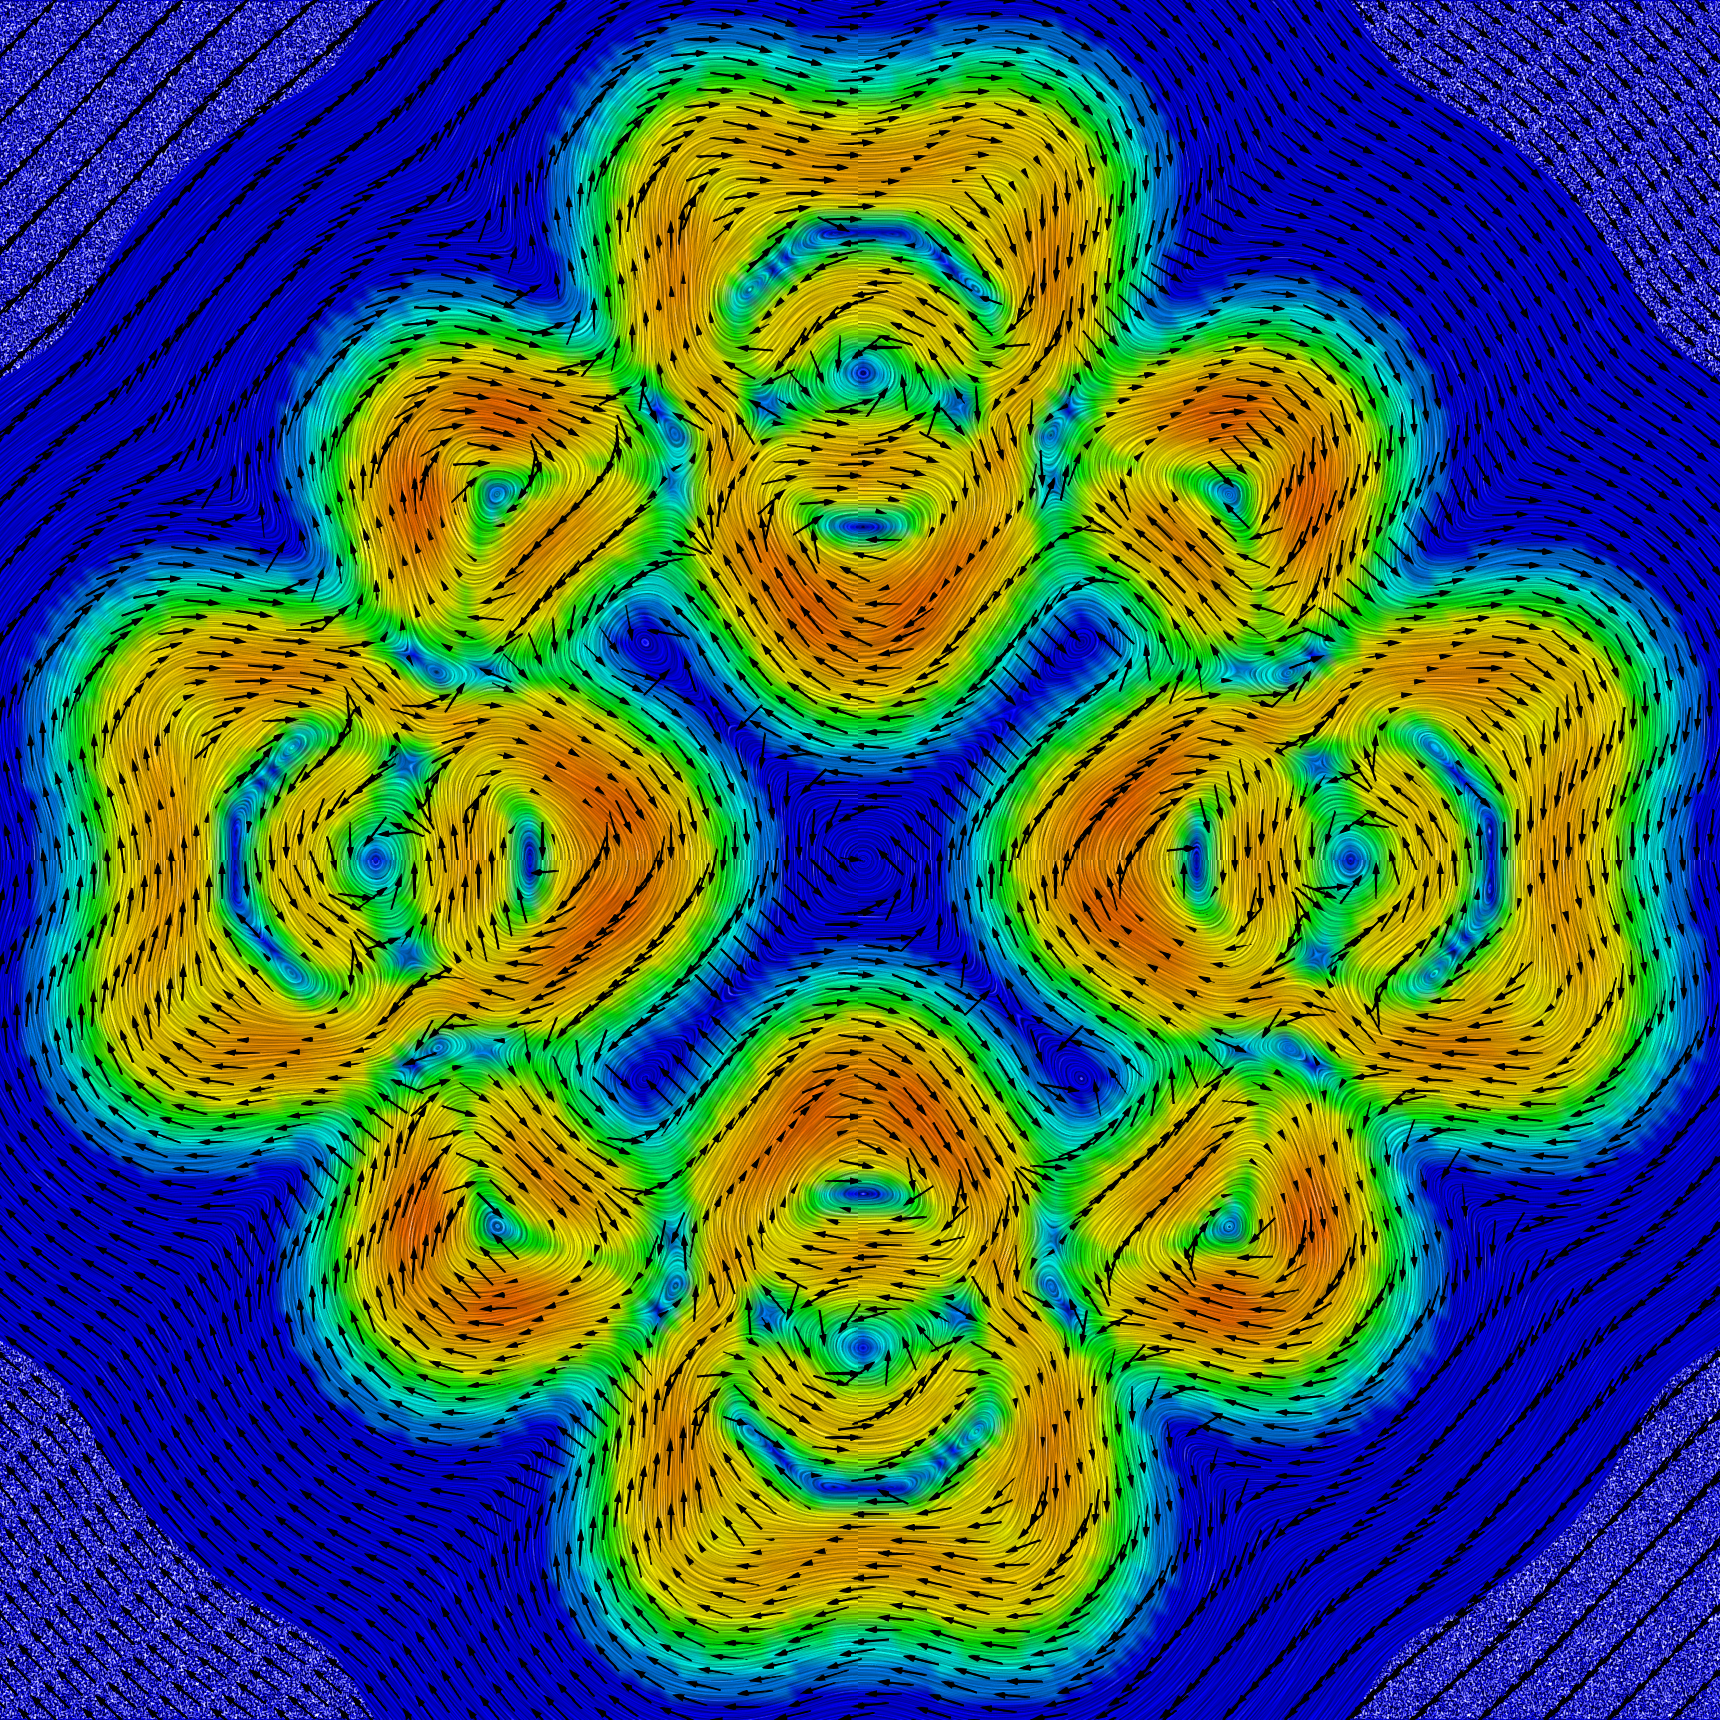
\includegraphics[width=0.6\textwidth]{b8s16_1bohr}
	\captionsetup{figurewithin = chapter}
	\captionsetup{font=small, labelfont=bf}\caption[Ringströme in B$_8$S$_{16}$]{Ringströme in B$_8$S$_{16}$ \unit[1]{bohr} oberhalb der Molekülebene, dargestellt zwischen \unit[0]{a.u.} (blau) und \unit[0.07]{a.u.}.}
\label{abb:b8s16hlic}
\end{figure}

\begin{figure}[ht!]
	\centering
	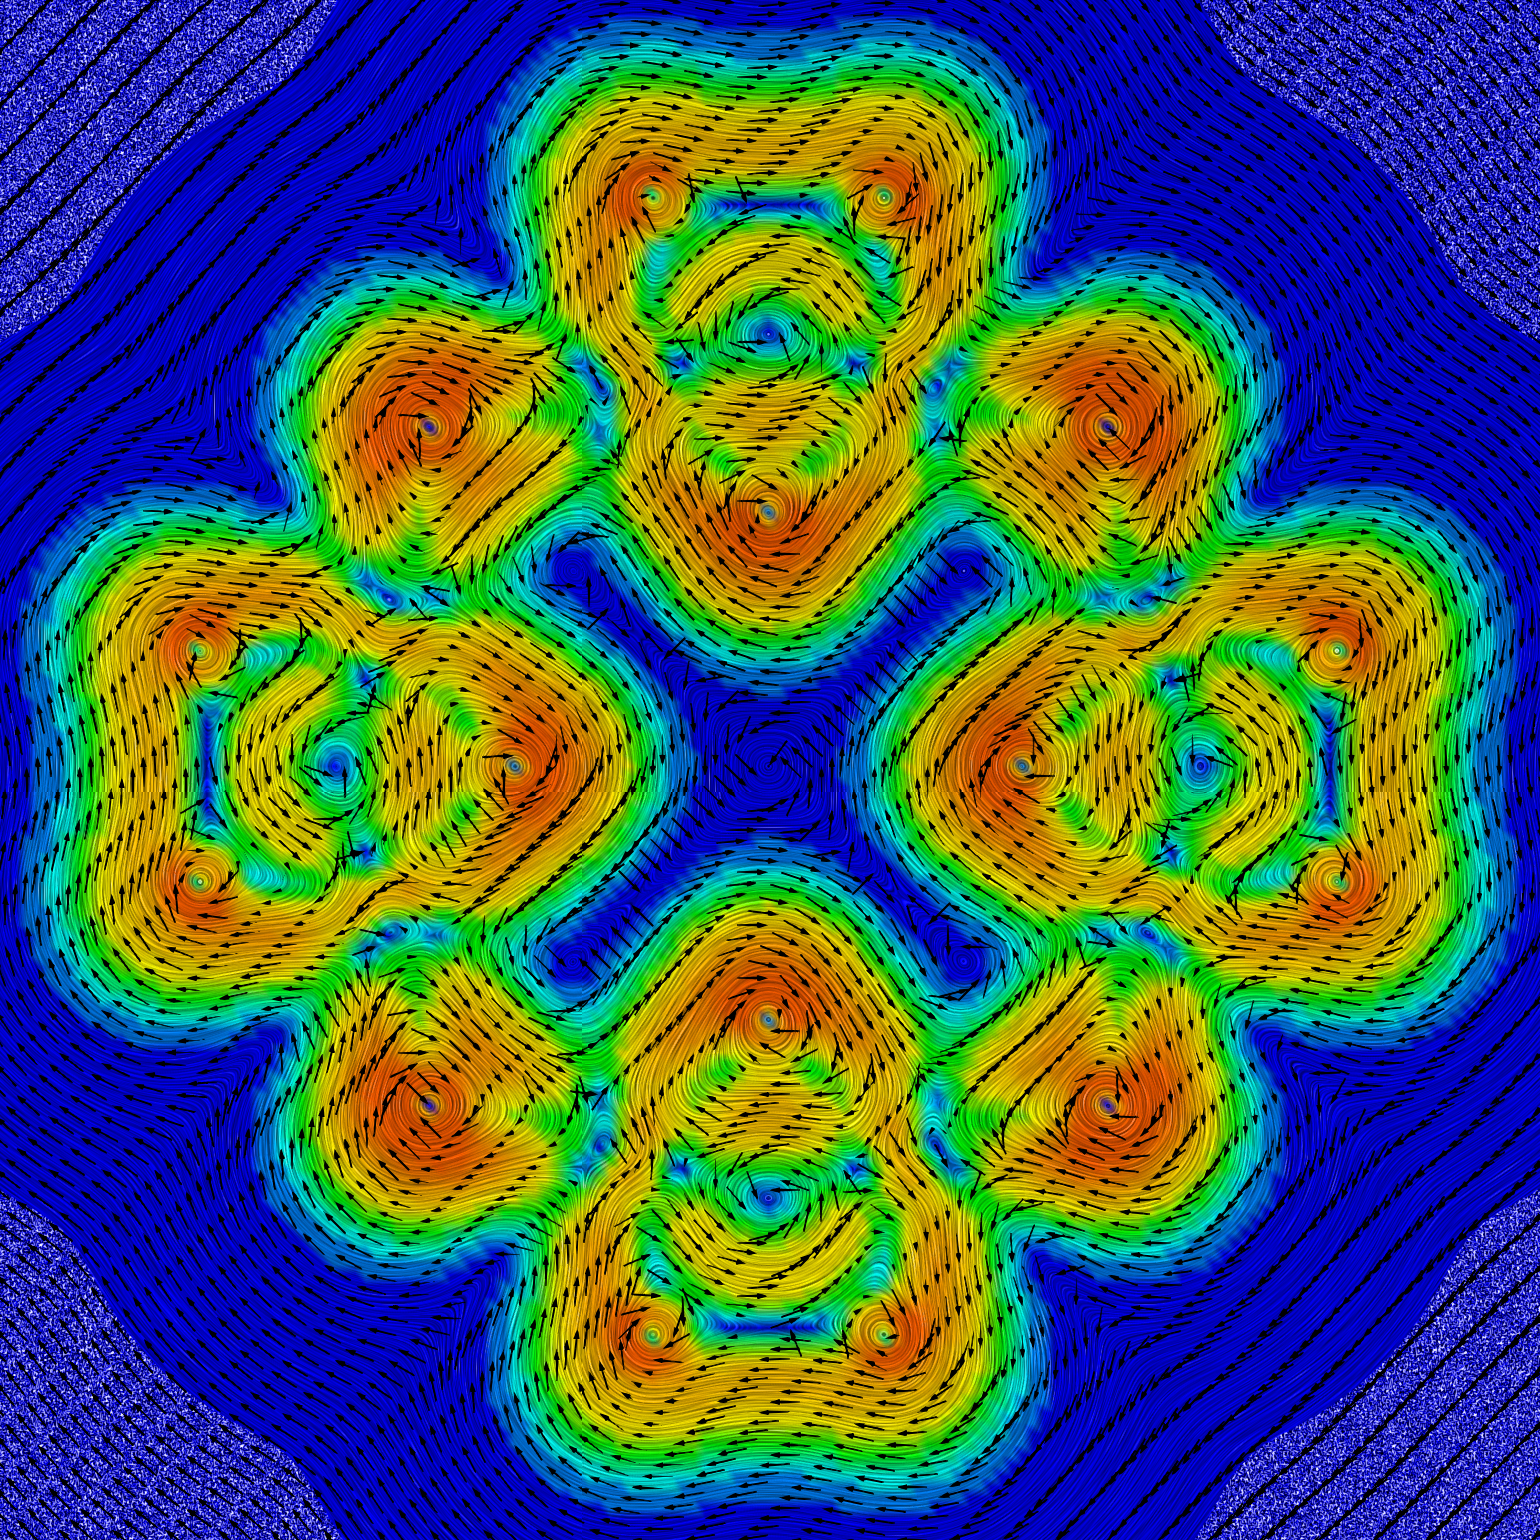
\includegraphics[width=0.6\textwidth]{b8se16_1bohr}
	\captionsetup{figurewithin = chapter}
	\captionsetup{font=small, labelfont=bf}\caption[Ringströme in B$_8$Se$_{16}$]{Ringströme in B$_8$Se$_{16}$ \unit[1]{bohr} oberhalb der Molekülebene, dargestellt zwischen \unit[0]{a.u.} (blau) und \unit[0.07]{a.u.}.}
\label{abb:b8se16hlic}
\end{figure}
\newpage
\subsection{[Co\@Sn$_6$Sb$_6$]$^{3-}$}
\newpage
\section{Ringströme in großen ringförmigen Kohlenstoffnanoröhren}